%Version 3 October 2023
% See section 11 of the User Manual for version history
%
%%%%%%%%%%%%%%%%%%%%%%%%%%%%%%%%%%%%%%%%%%%%%%%%%%%%%%%%%%%%%%%%%%%%%%
%%                                                                 %%
%% Please do not use \input{...} to include other tex files.       %%
%% Submit your LaTeX manuscript as one .tex document.              %%
%%                                                                 %%
%% All additional figures and files should be attached             %%
%% separately and not embedded in the \TeX\ document itself.       %%
%%                                                                 %%
%%%%%%%%%%%%%%%%%%%%%%%%%%%%%%%%%%%%%%%%%%%%%%%%%%%%%%%%%%%%%%%%%%%%%

%%\documentclass[referee,sn-basic]{sn-jnl}% referee option is meant for double line spacing

%%=======================================================%%
%% to print line numbers in the margin use lineno option %%
%%=======================================================%%

% \documentclass[lineno,sn-basic]{sn-jnl}% Basic Springer Nature Reference Style/Chemistry Reference Style

%%======================================================%%
%% to compile with pdflatex/xelatex use pdflatex option %%
%%======================================================%%

\documentclass[pdflatex,sn-basic, Numbered]{sn-jnl}% Basic Springer Nature Reference Style/Chemistry Reference Style

%%Note: the following reference styles support Namedate and Numbered referencing. By default the style follows the most common style. To switch between the options you can add or remove �Numbered� in the optional parenthesis.
%%The option is available for: sn-basic.bst, sn-vancouver.bst, sn-chicago.bst%

% \documentclass[sn-nature]{sn-jnl}% Style for submissions to Nature Portfolio journals
% \documentclass[sn-basic]{sn-jnl}% Basic Springer Nature Reference Style/Chemistry Reference Style
% \documentclass[sn-mathphys-num]{sn-jnl}% Math and Physical Sciences Numbered Reference Style
%%\documentclass[sn-mathphys-ay]{sn-jnl}% Math and Physical Sciences Author Year Reference Style
% \documentclass[sn-aps]{sn-jnl}% American Physical Society (APS) Reference Style
%\documentclass[sn-vancouver,Numbered]{sn-jnl}% Vancouver Reference Style
%%\documentclass[sn-apa]{sn-jnl}% APA Reference Style
%%\documentclass[sn-chicago]{sn-jnl}% Chicago-based Humanities Reference Style

%%%% Standard Packages
%%<additional latex packages if required can be included here>

\usepackage{graphicx}%
\usepackage{multirow}%
\usepackage{amsmath,amssymb,amsfonts}%
\usepackage{amsthm}%
\usepackage{mathrsfs}%
\usepackage[title]{appendix}%
\usepackage{xcolor}%
\usepackage{textcomp}%
\usepackage{manyfoot}%
\usepackage{booktabs}%
\usepackage{algorithm}%
\usepackage{algorithmicx}%
\usepackage{algpseudocode}%
\usepackage{listings}%
\usepackage{multicol}

% additional packages
\usepackage{caption}
\usepackage{placeins}
\usepackage{lipsum}
\usepackage{float}
\usepackage{csquotes}
\usepackage{sidecap}
\usepackage{url}                     % fix URL wrap
\usepackage{booktabs}                % Improves the quality of tables in LaTeX
\usepackage{tabularx}                % Enhances the standard LaTeX tables
\usepackage{subcaption}              % Provides support for subfigures and subtables
\usepackage{longtable}               % Allows the creation of multi-page tables
\usepackage{multirow}                % Enables cells spanning multiple rows in tables
\usepackage{threeparttable}          % Provides additional functionality for tables
\usepackage{array}
\usepackage{eurosym}

\def\UrlBreaks{\do\/\do-}
\renewcommand{\floatpagefraction}{0.5}
\renewcommand{\textfraction}{0.1}
%%%%%=============================================================================%%%%
%%%%  Remarks: This template is provided to aid authors with the preparation
%%%%  of original research articles intended for submission to journals published
%%%%  by Springer Nature. The guidance has been prepared in partnership with
%%%%  production teams to conform to Springer Nature technical requirements.
%%%%  Editorial and presentation requirements differ among journal portfolios and
%%%%  research disciplines. You may find sections in this template are irrelevant
%%%%  to your work and are empowered to omit any such section if allowed by the
%%%%  journal you intend to submit to. The submission guidelines and policies
%%%%  of the journal take precedence. A detailed User Manual is available in the
%%%%  template package for technical guidance.
%%%%%=============================================================================%%%%

%% as per the requirement new theorem styles can be included as shown below
\theoremstyle{thmstyleone}%
\newtheorem{theorem}{Theorem}%  meant for continuous numbers
%%\newtheorem{theorem}{Theorem}[section]% meant for sectionwise numbers
%% optional argument [theorem] produces theorem numbering sequence instead of independent numbers for Proposition
\newtheorem{proposition}[theorem]{Proposition}%
%%\newtheorem{proposition}{Proposition}% to get separate numbers for theorem and proposition etc.

\theoremstyle{thmstyletwo}%
\newtheorem{example}{Example}%
\newtheorem{remark}{Remark}%
\theoremstyle{thmstylethree}%
\newtheorem{definition}{Definition}%

\raggedbottom
%%\unnumbered% uncomment this for unnumbered level heads

\newcommand{\comment}[1]{\textcolor{purple}{#1}}

\begin{document}

\title[Article Title]{On the role of 24/7 carbon-free energy matching in accelerating advanced clean energy technologies}

%%=============================================================%%
%% GivenName	-> \fnm{Joergen W.}
%% Particle	-> \spfx{van der} -> surname prefix
%% FamilyName	-> \sur{Ploeg}
%% Suffix	-> \sfx{IV}
%% \author*[1,2]{\fnm{Joergen W.} \spfx{van der} \sur{Ploeg}
%%  \sfx{IV}}\email{iauthor@gmail.com}
%%=============================================================%%

\author*[1]{\fnm{Iegor} \sur{Riepin}}\email{iegor.riepin@tu-berlin.de}
\author[1]{\fnm{Tom} \sur{Brown}}\email{t.brown@tu-berlin.de}
\author[2]{$<Princeton-team?>$}\email{$<Princeton?>$}
\author[3]{\fnm{Devon} \sur{Swezey}}\email{dswezey@google.com}

\affil[1]{\orgdiv{Department of Digital Transformation in Energy Systems}, \orgname{TU Berlin}, \orgaddress{Germany}}

\affil[3]{\orgdiv{Global Energy and Climate}, \orgname{Google LLC}}

%%==================================%%
%% Sample for unstructured abstract %%
%%==================================%%

\abstract{

Commitments to 24/7 carbon-free energy matching by companies and governments create an early market for advanced energy technologies like long-duration energy storage and clean firm generators that fill the gaps between wind and solar generation.
We argue that the commitment by a small number of companies to round-the-clock matching can spur substantial technological learning in advanced technologies, leading to cost reductions \comment{of up to 44\%}. 
This makes 24/7 matching more attractive for other actors, leading to a virtuous circle that accelerates the point where the technologies become cost-competitive in the rest of the electricity market. 
These indirect effects unlock greenhouse gas savings far beyond the direct avoidance of the initial investments.
}

% \keywords{keyword1, Keyword2, Keyword3, Keyword4}

%%\pacs[JEL Classification]{D8, H51}

%%\pacs[MSC Classification]{35A01, 65L10, 65L12, 65L20, 65L70}

\maketitle

\subsection*{Big challenges ahead}\label{sec1}

Tackling climate change requires not only a massive scale-up of available energy technologies like wind, solar and batteries, but also an accelerated research, development, demonstration (RD\&D) and widespread deployment of advanced technologies that are not yet commercialised at scale \cite{sepulvedaRoleFirmLowCarbon2018, bistlineImpactCarbonDioxide2021, brownUltralongdurationEnergyStorage2023, ieaNetZero20502021}.
Among them are clean firm generation technologies, such as next-generation geothermal power, advanced nuclear generators, Allam-cycle gas generators with carbon capture and storage (CCS), as well as long-duration energy storage (LDES) technologies, which can bridge gaps in clean power supply for a few days to weeks that cannot be filled by wind, solar photovoltaics (PV), or batteries.

\textbf{Barriers to commercialization---} Bringing new technologies to market on a large scale and in time, however, is fraught with big challenges.
New technologies often face a \enquote{valley of death} on the path from the development stage to successful commercial deployment \cite{gatesFinancingCleanIndustrial2021, google-advancedtech}.
Companies developing a new technology must first prove that it works safely and reliably at pilot scale.
One major hurdle at this stage is the scarcity of financing. Early-stage investments typically comprise R\&D grants and venture capital, insufficient in both magnitude and duration to support new energy technologies. On the other hand, mature technologies such as wind and solar attract steady, de-risked capital from institutional investors \cite{google-advancedtech, khatcherianBarriersTimelyDeployment2022}.

After that, companies must construct larger plants at sufficient scale and manufacturing cost to achieve commercial viability. This requires overcoming financial, engineering, and supply chain issues that come with building a first-of-its-kind (FOAK) project, and afterward optimizing processes to gradually cut the costs. Technology innovators frequently lack the expertise to scale from small demonstration plants to commercial-scale projects. Often, moving through this milestone requires a consortium of stakeholders, increasing project complexity and risk, thereby complicating financing \cite{google-advancedtech}.
Even when FOAK technologies are successfully demonstrated, scaling to subsequent projects remains difficult. New technologies must be repeatedly deployed to achieve economies of scale and reduce costs. However, procurement typically focuses on individual plants rather than larger portfolios, with many observers preferring to \enquote{wait and see} how the new generation of a technology performs before committing to an investment. Overall, the road from the first demonstration plant to commercial uptake can be complicated, risky, and expensive---and it is challenging to secure the capital to fund it.

\textbf{Bridging the valley of death---} Consider how solar became global industry and a truly disruptive technology. Bell Labs developed the first silicon photovoltaic cell in 1954, which made modern solar power possible. After more than 20 years of further development, in 1975, the Levelised Cost of Electricity (LCOE) for solar PV was above \$10.000/MWh. A historical trajectory for solar development involves Japans's niche markets for consumer electronics in the 1980s, and Germany's feed-in tariff in 2004, which created a \enquote{demand pull} that significantly drove down costs through technological learning \cite{nemetHowSolarEnergy2019}. Fast forward to 2020s, for projects with low-cost financing that tap high-quality resources, solar PV is now \textit{the cheapest source of electricity in history}, with new utility-scale solar projects cost at \$30-60/MWh in Europe and the US and just \$20-40/MWh in China and India \cite{WorldEnergyOutlook2020}.

However, it took \textit{six decades} for solar to become economically viable. The urgency of the climate crisis demands that we accelerate this process for advanced clean electricity technologies. A crucial question here: Who will invest in these technologies when they are expensive at the beginning? Understanding the wider social benefit of such investments is another important aspect.  New technologies, such as Allam cycle generators and iron-air battery storage, have characteristics that make them suitable for following solar's path. They benefit from evolving R\&D process, learning by doing and iterative upscaling. In this way, even though initial investments come with a price premium and certain risks, they can result in cost reductions and an earlier rollout of advanced clean energy technologies. In turn, this produces indirect effects that unlock greenhouse gas savings far beyond the direct avoidance associated with the initial investments.

\subsection*{The significance of 24/7 CFE matching}\label{sec2}

Many public and private energy buyers support the global effort to decarbonise electricity systems by purchasing clean energy.
An increasing number of buyers are adopting the most ambitious approach to clean energy purchasing, aiming to eliminate \textit{all carbon emissions} associated with their electricity use.
This approach is called the 24/7 Carbon-Free Energy (CFE) matching, i.e., aligning electricity demand with carbon-free energy energy supply on \textit{an hourly basis}.
24/7 CFE commitments were announced by large technology companies such as Google, Microsoft and IronMountain \cite{google-247by2030, Microsoft-vision, IronMountainSustainability}, as well as by utilities \cite{peninsula-OurPathto247}, the US federal government \cite{thewhitehouseExecutiveOrderCatalyzing2021}, and some city governments \cite{iowaenvcouncil-247}.
% In 2021, an international group of stakeholders launched the 24/7 Carbon-free Energy Compact \cite{gocarbonfree247}. With over 150 signatories, the group aims to develop and scale high-impact technologies, energy policies, procurement practices, and solutions to make 24/7 Carbon-Free Energy achievable for all.

Motivated by these commitments, several quantitative studies have been conducted on the means, costs, and system-level impacts of hourly CFE matching \cite{xu-247CFE-report, ieaAdvancingDecarbonisationClean2022, riepin-zenodo-systemlevel247, riepinMeansCostsSystemlevel2024}. There are three key findings that emerge from these studies:
\begin{enumerate}
    \item 24/7 CFE commitments reduce participating buyers' emissions as well as emissions from the electricity grids where they operate.
    \item 24/7 CFE comes at a cost premium for participating consumers if only mature technologies, such as solar PV, wind, and battery storage, are used for CFE sourcing.
    \item The cost premium can be substantially reduced if participating buyers incorporate a broad range of advanced energy technologies into their procurement strategies, such as long-duration energy storage and clean firm generators.
\end{enumerate}

\textbf{An illustrative example---} We reproduce the three findings above in an example depicted in Fig. \ref{fig:dashboard}.
Here we display a situation in which a fraction of electricity demand in a particular bidding zone (here---Germany) voluntarily commits to matching their electricity demand with carbon-free electricity round-the-clock.
Hereinafter, the participating demand is referred to as \enquote{participating consumers}.
Panel A illustrates the intuition---once demand and supply are perfectly aligned on an hourly basis, participating consumers reach zero emission rate (gCO$_2$/kWh$^{-1}$) attributed to their electricity consumption. This goal requires a large portfolio of wind, solar PV, and batteries, as shown in Panel B. It is indeed difficult to match every kWh of electricity consumption with renewable electricity during times of dark wind lulls. As a result, achieving 24/7 CFE matching, including the most difficult 2\% of times, adds a high cost premium for consumers in part due the need to overbuild capacity relative to the demand of participating buyers (\enquote{p1-cfe100}). Finding \#3 above is also clearly visible in Panel C: the power capacity required for 24/7 CFE matching and associated costs are substantially reduced when LDES technology (iron-air battery storage) or clean firm generation technologies (Allam cycle generator with CCS) are added.

\begin{figure}[htbp]
    \centering
    \includegraphics[width=\textwidth]{images/dashboard_1.pdf}
    \captionsetup{width=\textwidth}
    \caption{Illustrative modelling of 24/7 CFE matching.
    \textbf{Panel a}: Average emissions rate of participating consumers,
    \textbf{panel b}: portfolio capacity procured by participating consumers,
    \textbf{panel c}: procurement cost by scenario.
    Here we assume Germany 2025 as an example location and participation rate of C\&I consumers in 24/7 CFE matching strategy at 5\% (ca. 1900~MW load).
    CFE scores 90\%, 98\% and 100\% correspond to the share of time when the electricity consumed by the participating consumers is carbon-free.
    P1: palette of technologies that are commercially available today: onshore wind, utility scale solar PV, and battery storage; P2: all above plus iron-air battery storage; P3: all above plus an Allam cycle generator. The 24/7 CFE procurement framework is based on the methodologies paper by \citet{google-methodologies}. Simulations were carried out using the 24/7 CFE model by \citet{riepin-zenodo-systemlevel247}. Technology assumptions are provided in Table \ref{tab:tech_costs}.\\
    }\label{fig:dashboard}
\end{figure}

The key observation from Fig. \ref{fig:dashboard} can be summarized as follows: \textit{24/7 CFE commitments create an early market for advanced clean electricity technologies, which reduce the costs of hourly CFE matching}. If only 5\% of commercial and industrial (C\&I) consumers in Germany---representing approximately 1900~MW of load---adopt 24/7 CFE matching strategy, this would create a market for approximately 1500~MW of advanced clean firm generators and about 23~GWh of long-duration energy storage (\enquote{p3-cfe100}, Fig. \ref{fig:dashboard}). In similar vein how feed-in tariffs and renewable portfolio standards created a \enquote{demand pull} for wind and solar technologies in the past, 24/7 CFE commitments can drive the deployment and accelerate innovation of advanced clean electricity technologies.

\FloatBarrier
\subsection*{Technology learning}\label{sec3}

The early deployment of advanced clean electricity technologies can help them drive down along the \enquote{experience curve} -- a concept encapsulating a set of mechanisms by which technology specific costs decline as cumulative capacity is developed: evolving R\&D process, learning-by-doing, incremental upscaling, economies of scale, financial innovation and experience, for example.

In this section, we analyse the expected technological learning for two advanced technologies that were developed as a result of 24/7 CFE commitments: the Allam cycle generator and the iron-air battery storage system. The mathematical model of learning is based on empirical evidence in which the specific investment costs $C$ of a technology decrease by a constant factor with each doubling of experience $E$ \cite{wayEmpiricallyGroundedTechnology2022a}. The functional dependency is given by:

\begin{equation}
  \begin{aligned}
    \color{violet}C(E)\color{black} &= \color{blue}\overline{C_0}\color{black}  \cdot \left( \frac{\color{red}E}{\color{blue}\overline{E_0}\color{black}} \right)^{-\color{black}\alpha} \text{ where } \color{black}\alpha = \color{black}\log_2 \left( \frac{1}{1 - \color{blue}LR\color{black}} \right)
    \label{eq:learning_curve}
  \end{aligned}
\end{equation}

\noindent where the constants $\color{blue}\overline{C_0}$ [\officialeuro/kW] and $\color{blue}\overline{E_0}$ [MW] are fixed starting points representing the initial costs and experience levels, respectively. The learning rate $\color{blue}LR$ [\%] is a parameter that determines the rate at which costs decrease with experience. If $\color{blue}LR=20\%$, the costs are reduced by 20\% for each doubling of cumulative experience. Typically learning rates range between 5\%--25\% \cite{waySuppplementaryMaterialsEmpirically2022}. Here we use cumulative capacity $\color{red}E$ [MW] of a technology as a proxy for experience, which is calculated as the sum of the installed capacities of all projects that have been completed by a certain point in time. We collect information on existing and planned project for each technology, and use this as a starting point for the experience of the technology. 24/7 CFE matching contributes to the technology's experience the additional capacity procured by participating consumers, which is proportional to the participation rate (i.e., the share of electricity demand that is matched with carbon-free electricity on an hourly basis).

The resulting investment costs $\color{violet}C(E)\color{black}$ [\officialeuro/kW] are shown in Fig. \ref{fig:panels} for Allam cycle technology (top panel) and iron-air battery storage (bottom panel).
The first 1\% of participation (around 380~MW load in the German market) reduces costs for Allam cycle generators by 9\% and iron-air storage by 16\%. The technology learning scales significantly from there: at 10\% participation, Allam cycle generators and iron-air storage cost are reduced by 35\% and 45\%, respectively. The learning effect has a diminishing return, due to the logarithmic term $\color{black}\alpha$ in Eq. \ref{eq:learning_curve}. In other words, the first projects have the most significant impact on technology learning, and the effect diminishes as technology experience grows. \\


\noindent\textbf{on signal-to-noise} there is much uncertainty behind this back-of-the-envelope calculation. Assumptions on the initial capacity, costs and Learning Rate drive the results. We'll capture and visualise the parametric uncertainty as follows by running monte carlo analysis on initial experience/costs ($\color{blue}\overline{E_0}\color{black}$/$\color{blue}\overline{C_0}\color{black}$) and assuming a broad range of learning rates 15$\pm$5\%. \\


Parametric uncertainty has an impact on the results, which we capture in the Monte Carlo simulation panel. The key outcome is robust to uncertainty: Voluntary commitments to the hourly matching accelerate electricity system transformation through an early deployment of advanced energy technologies. \\


\begin{figure}[htbp]
    \centering
    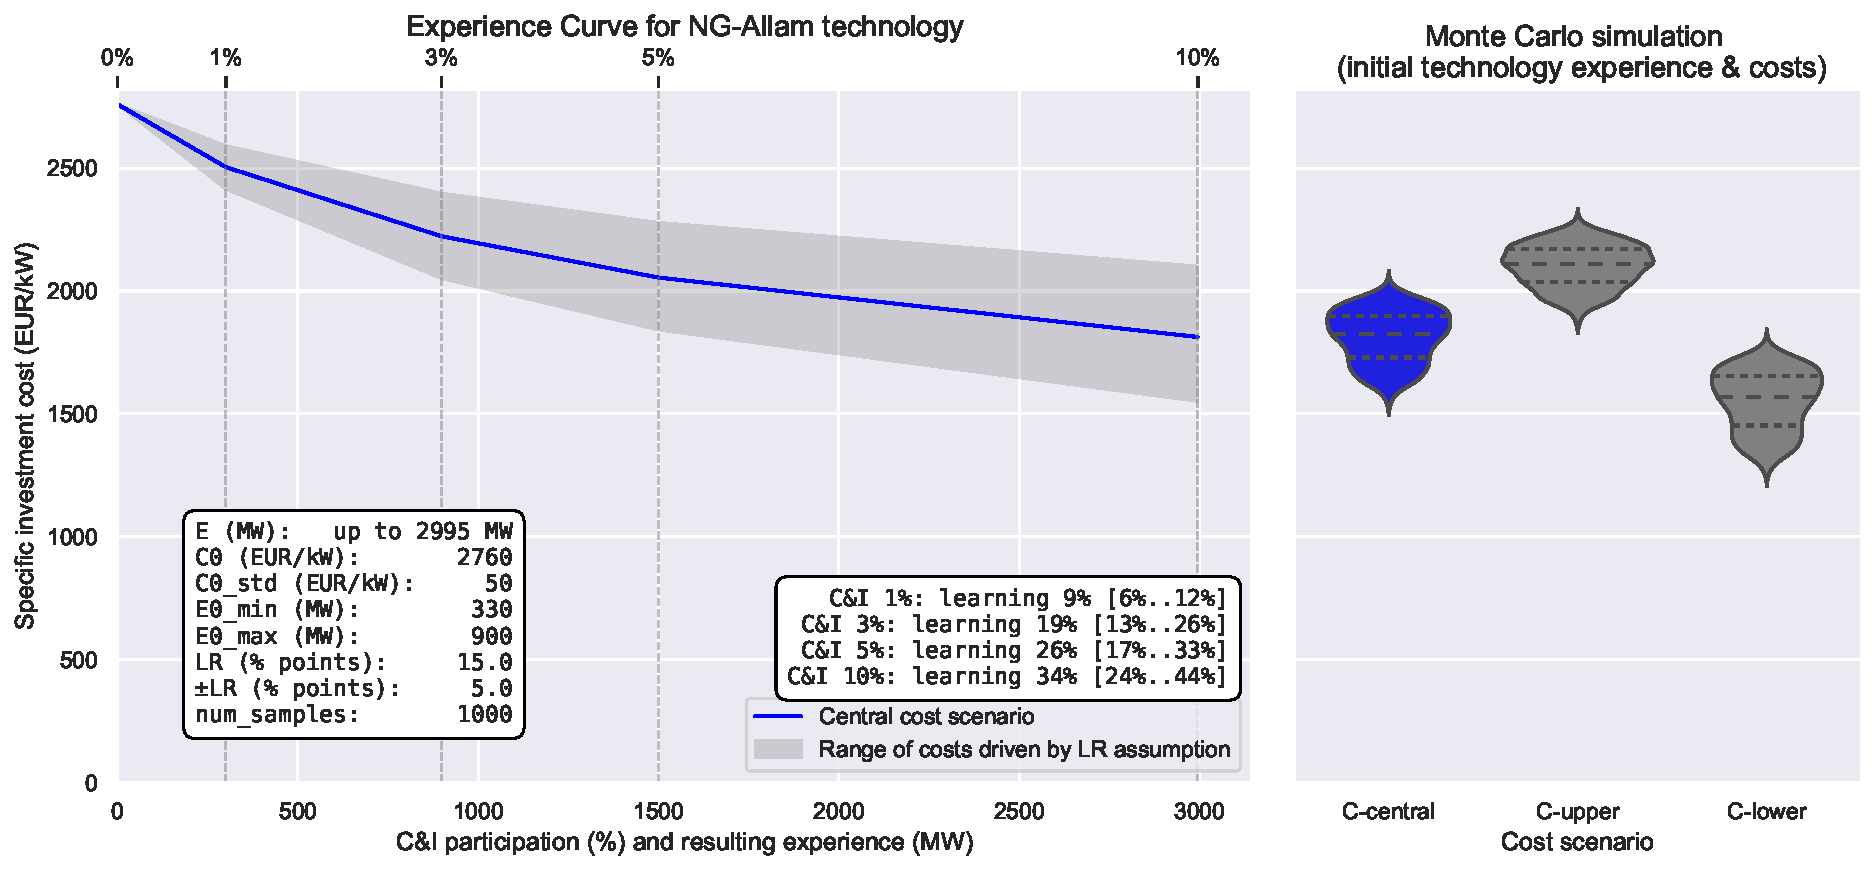
\includegraphics[width=\textwidth]{images/e_curve_NG-Allam.pdf}
    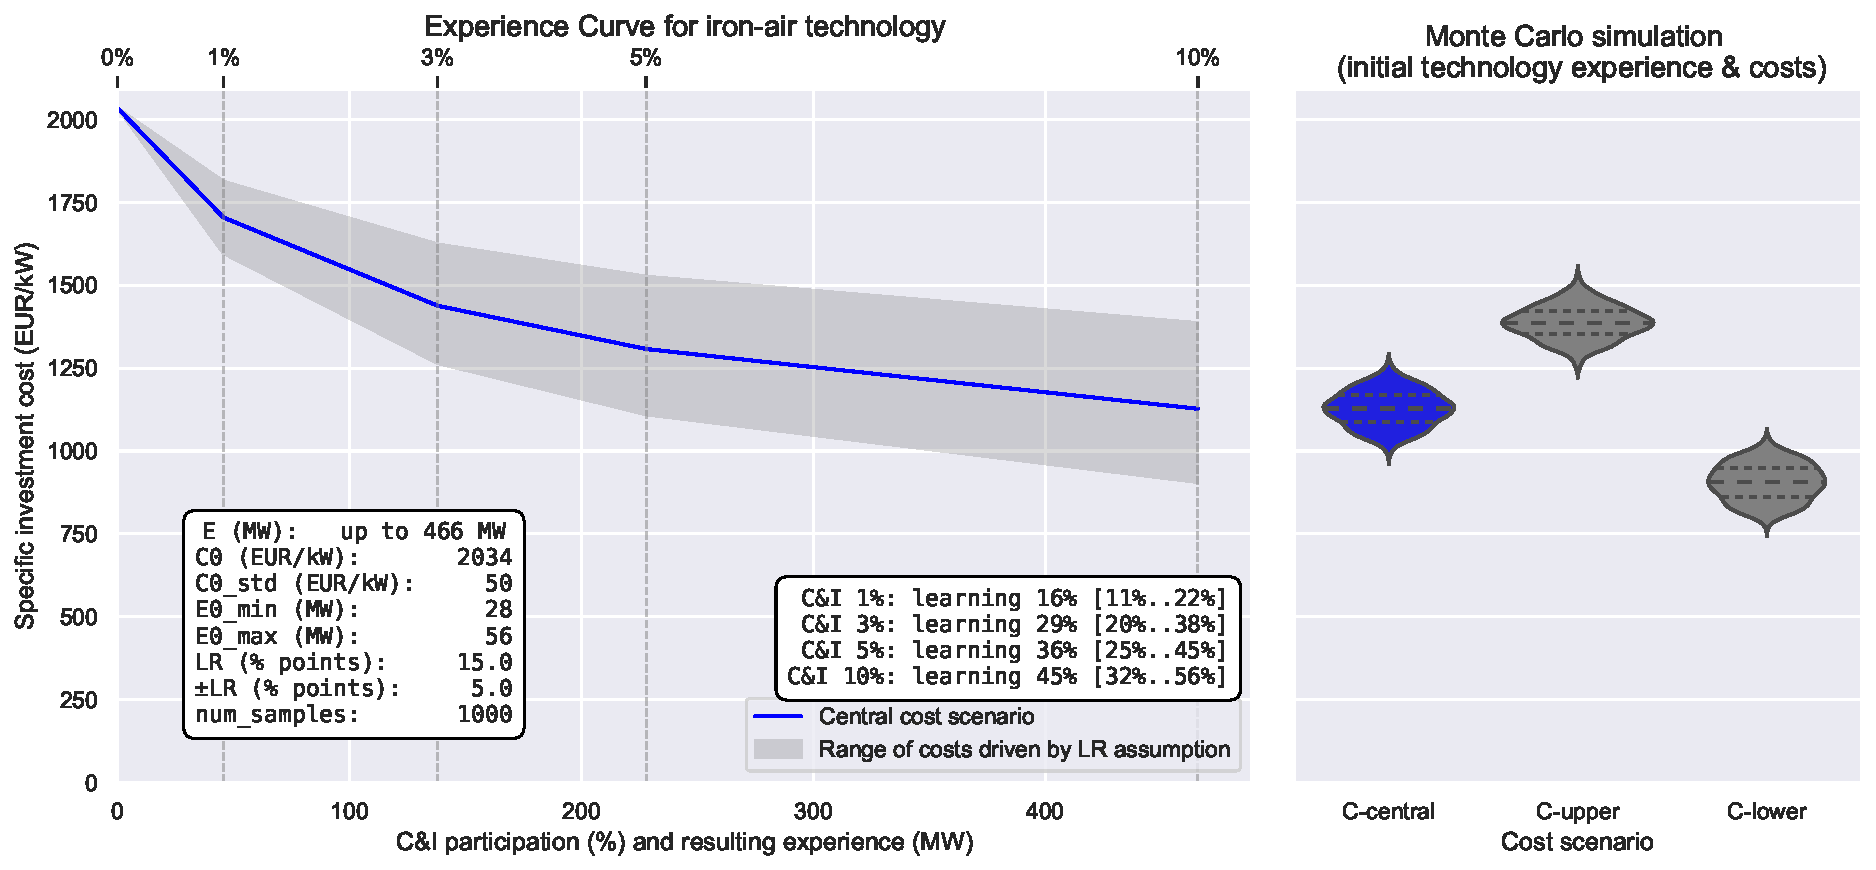
\includegraphics[width=\textwidth]{images/e_curve_iron-air.pdf}
    \caption{Technology learning curves for the NG-Allam cycle (\textbf{top panel}) and iron-air battery storage (\textbf{bottom panel}).
    The learning curves are based on the experience model with the technology investments based on 24/7 CFE model with varying C\&I participation level $[0\%..10\%]$ and learning rates of 15$\pm$5\%.
    For the Monte Carlo analysis calibration, the initial costs (C0) are sampled from a normal distribution with a mean based on technology cost assumptions for 2025 and a standard deviation of 50~EUR/kW. Initial experience levels (E0) are sampled from a uniform distribution, with bounds derived from public information about planned projects. In NG-Allam's model, initial experience lies between cases when one of three planned projects planned by 2025 is completed, and when all three projects are completed \cite{BroadwingEnergyProject, CoyoteCleanPower, FrogLakeProject}. In iron-air storage model, the distribution bounds are formed by assuming that 50\% to 100\% of the projects announced to operate by 2025 are realized on time \cite{FormEnergyLatest2024}.
    }
    \label{fig:panels}
\end{figure}

\subsection*{System impact}\label{sec3}

\comment{Here story goes as follows}

Reduced cost for advanced technologies facilitate decarbonisation of electricity systems through several channels:

First, 24/7 CFE has direct decarbonisation impact through two individual mechanisms -- profile and volume, see Priceton (2022) and Riepin \& Brown (2023) for detail. Note that profile mechanism makes 24/7 CFE impactful even in clean regions and future times.

Second, early commitments to 24/7 CFE facilitate innovation and create the early market for advanced technologies, as shown above. More companies can join 24/7 CFE movement due to reduced price premium.  This in turn lowers system emissions via the two mechanisms above.

Third, at some point, advanced technologies break even economically in the background grid, as shown in Fig. \ref{fig:impact}:

\begin{itemize}
    \item Figure shows that iron-air battery storage enters optimal investment mix with CAPEX ~1525 EUR/kW (75\% cost reduction).
    \item System emissions drop because iron-air substitute fossil peakers (gas OC), and later facilitates efficient use of RES excess.
    \item This CAPEX point is crossed if existing 2025 capacity of iron-air battery \textbf{is doubled twice}, what can be derived from Fig. \ref{fig:panels}. \\
    (here I have to simplify across multiple data points depending on realisation of E0, C0 and LR. Simply put, it needs roughly 2x expected capacity by 2025 and LR [0.10 .. 0.15].)
    \item In other words, it requires \textbf{0.35B investment} to bring iron-air experience to the point of economical break-even in the background grids by 2030. \\
    (170 MW * 2034 EUR/kW * 1e3 ) / 1e9)
    \item This learning can be reached if C\&I consumers with aggregated demand of ca. 1200MW join 24/7 CFE movement -- that is 3\% of C\&I in DE sector. NB! That learning effect can be reached with even lower participation, if C\&I consumers focus their investment strategies on LDES (iron-air).
\end{itemize}

\begin{figure}[htbp]
    \centering
    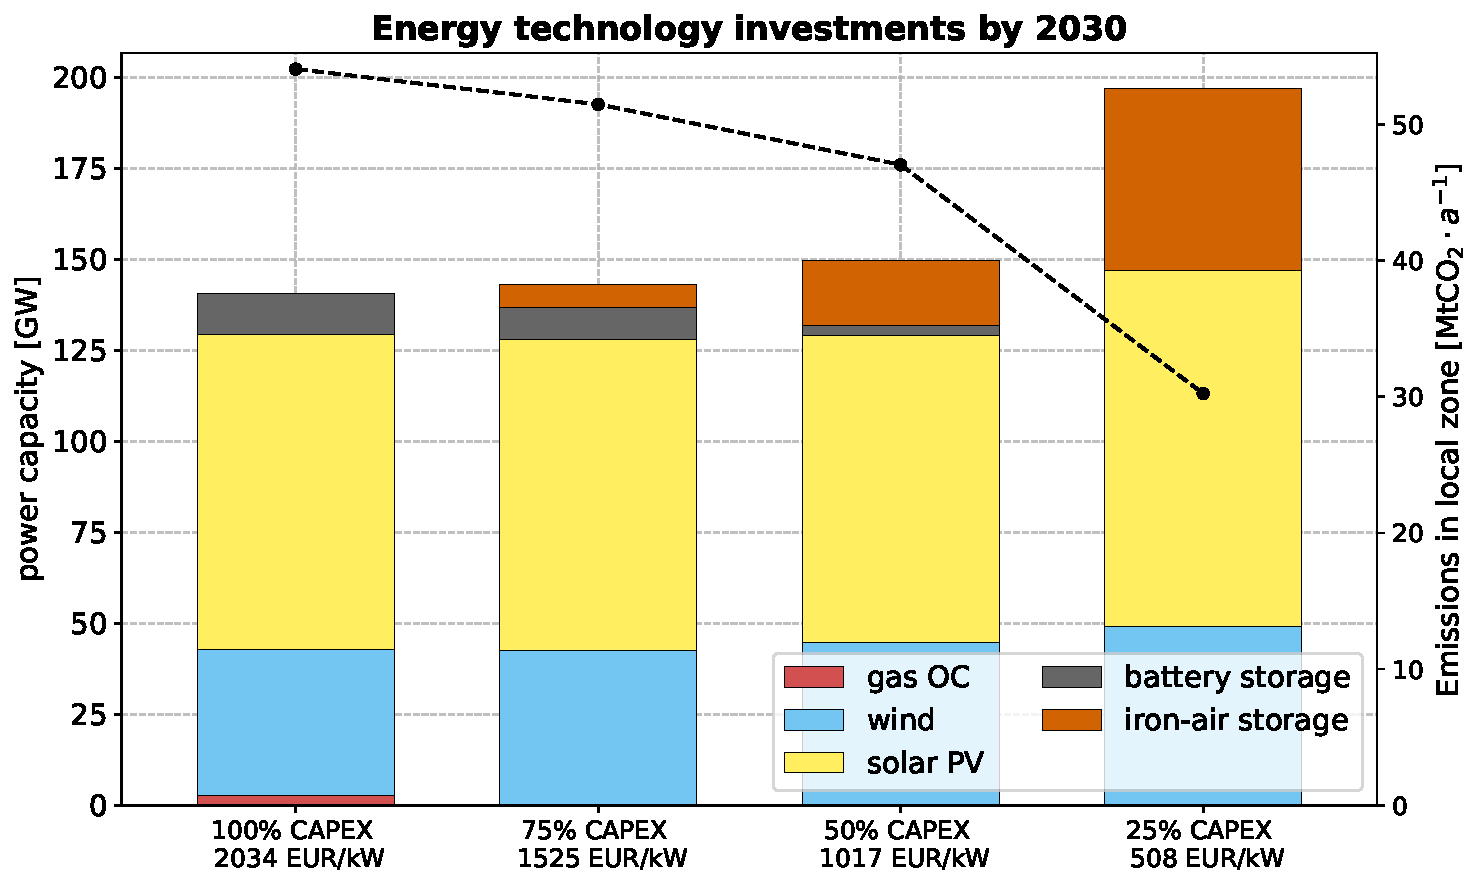
\includegraphics[width=0.8\textwidth]{images/dashboard_3.pdf}
    \caption{Power capacity investments and emissions in German 2030 electricity system as a function of CAPEX for iron-air storage. Here iron-air storage has a fixed duration of 100 hours \cite{FormEnergyLatest2024}. Price for EU ETS allowances is 100 EUR/tCO$_2$. Technology costs are based on DEA \cite{DEA-technologydata}. Other background system assumptions are aligned with \citet{riepin-zenodo-systemlevel247}.}\label{fig:impact}
    \captionsetup{width=0.3\textwidth}  % Adjust according to your needs
\end{figure}


\subsection*{A broad perspective}\label{sec4}

\comment{A short 1 paragraph conclusion goes as follows}

Reduced costs of advanced clean electricity technologies benefits all: \\
-- lower costs for 24/7 CFE matching for followers \\
-- makes deep decarbonization more affordable and enables more ambitious climate goals \\
-- facilitates energy security and resilience \\
-- reduce curtailment, and the need for transmission and distribution infrastructure 
Companies and governments optimizing their energy procurement and investment strategies to match own consumption with clean electricity round-the-clock can play a catalytic role in innovation, financeability, and widespread availability of technologies required for a wider societal transition to secure, reliable and clean energy systems.

% We find that 24/7 matching is a viable and effective strategy for electricity buyers aiming to eliminate their own carbon footprint and contribute to wider system decarbonisation.
% Voluntary commitments to the hourly matching strategy have a further transformative effect on electricity systems through accelerated innovation and early deployment of advanced energy technologies

%%%%%%%%%%%%%%%%%%%%%%%%%%%%%%%%%%%%%%%%%%%%%%%%%%%%%%%%
\backmatter

\bmhead{Acknowledgements} We thank the following people for insights and fruitful discussions: Elisabeth Zeyen, Adam Forni, Brian Denvir, and the participants of the 24/7 CFE Hub Meeting in May 2024. IR acknowledges a research grant from Google LLC.

\bmhead{Author contributions} The authors contributed equally to this work.

\bmhead{Code availability} The code to reproduce the illustrative experiments is available at GitHub under open licenses \cite{code247CFE}.

\bmhead{Competing interests} \comment{I suppose there is no competing interests to declare for this work from @TUB side, TB do you agree? @DS please suggest your line here.}


%%===========================================================================================%%
%% If you are submitting to one of the Nature Portfolio journals, using the eJP submission   %%
%% system, please include the references within the manuscript file itself. You may do this  %%
%% by copying the reference list from your .bbl file, paste it into the main manuscript .tex %%
%% file, and delete the associated \verb+\bibliography+ commands.                            %%
%%===========================================================================================%%

\bibliography{sn-bibliography}% common bib file
%% if required, the content of .bbl file can be included here once bbl is generated
%%\input sn-article.bbl

\FloatBarrier
\newpage 

\subsection*{Technology assumptions for the illustrative example of 24/7 CFE matching}
\label{sec:annex}

Cost and other assumptions for energy technologies available for 24/7 CFE participating consumers are collected from the Danish Energy Agency \cite{DEA-technologydata}.
Data for advanced clean firm technologies is less reliable due to technological uncertainty and lack of commercial experience; therefore, we use publicly available information and own estimates.
A full list of technology assumptions, including the data for energy technologies in the background energy system, is available via the reproducible scientific workflow in the GitHub repository \cite{code247CFE}.

\begin{table*}[h]
    \centering
    \resizebox{\textwidth}{!}{%
        \begin{tabular}{lccccccc}
            \hline\hline
            \textbf{Technology} &
            \textbf{Year} &
            \textbf{\begin{tabular}[c]{@{}c@{}}CAPEX\\ (overnight cost)\end{tabular}} &
            \textbf{\begin{tabular}[c]{@{}c@{}}FOM\\ {[}\%/year{]}\end{tabular}} &
            \textbf{\begin{tabular}[c]{@{}c@{}}VOM\\ {[}Eur/MWh{]}\end{tabular}} &
            \textbf{\begin{tabular}[c]{@{}c@{}}Efficiency\\ {[}per unit{]}\end{tabular}} &
            \textbf{\begin{tabular}[c]{@{}c@{}}Lifetime\\ {[}years{]}\end{tabular}} &
            \textbf{Source} \\ \hline\hline
            Utility solar PV & 2025 & 612 \officialeuro/kW & 1.7 & 0.01 & - & 37.5 & \cite{DEA-technologydata} \\
            Onshore wind & 2025 & 1077 \officialeuro/kW & 1.2 & 0.015 & - & 28.5 & \cite{DEA-technologydata} \\
            Battery storage & 2025 & 187 \officialeuro/kWh & - & - & - & 22.5 & \cite{DEA-technologydata} \\
            Battery inverter & 2025 & 215 \officialeuro/kW & 0.3 & - & 0.96 & 10 & \cite{DEA-technologydata} \\
            Iron-air storage & 2025 & 2034 \officialeuro/kW$^1$ & 1 & - & 0.43$^2$ & 15 & \cite{FormEnergyLatest2024} \\
            Allam cycle generator & 2025 & 2760 \officialeuro/kW$^3$ & 14.8 & 3.2 & 0.54 & 30 & \cite{navigant-report, NetZeroAmerica-report} \\
            \hline \hline
        \end{tabular}%
    }
\begin{tablenotes}
    {\small
    \item[] Notes: $^1$iron-air storage has a fixed duration of 100h, costs comprise both power and energy components; $^2$cycle efficiency, the model factors in efficiency factor of 0.71 for charge process and 0.60 for discharge; $^3$costs also include estimate of 40 \officialeuro/tCO$_2$ for carbon transport and sequestration; all costs are in 2023 euros; CAPEX = capital expenditure; FOM = fixed operations and maintenance costs; VOM = variable operations and maintenance costs.
    }
\end{tablenotes}
    \vspace{0.2cm}
    \caption{Technology assumptions.}
    \label{tab:tech_costs}
\end{table*}

\end{document}
